\documentclass[border=10pt]{standalone}

\usepackage{tikz}
\usepackage{tikzsymbols}
\usetikzlibrary{calc,patterns,shapes.geometric}

\def\centerarc[#1](#2)(#3:#4:#5){\draw[#1] ($(#2)+({#5*cos(#3)},{#5*sin(#3)})$) arc (#3:#4:#5);}

\begin{document}
	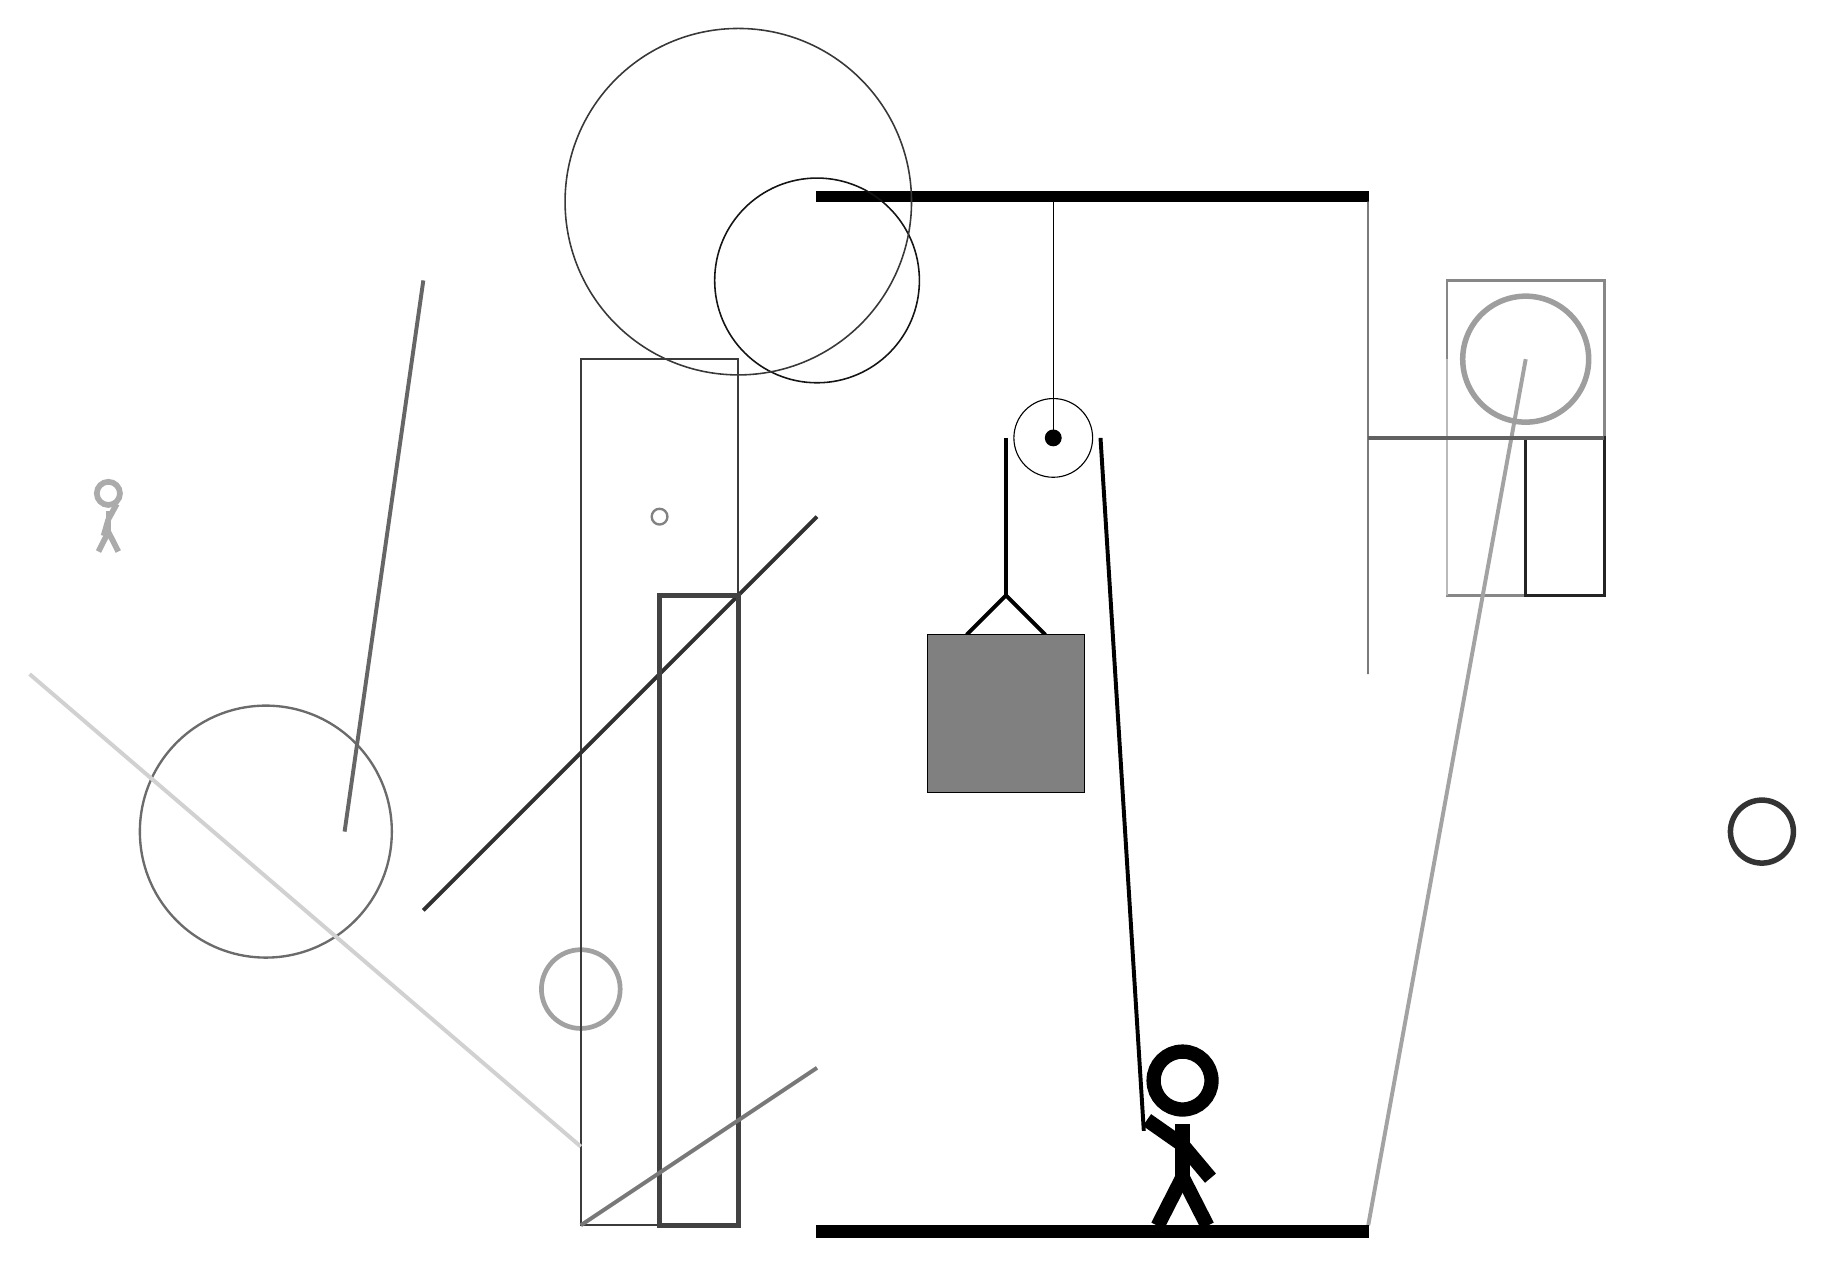
\begin{tikzpicture}
		%%%%% START %%%%%
		
		\draw[fill=black] (-2, 10) rectangle (5, 10.125);
		
		\draw (1, 7) circle (0.5);
		\draw[fill=black] (1, 7) circle (0.1);
		\draw (1, 10) -- (1, 7);
		
		\draw[line width=0.5mm] (-0.1, 4.5) -- (0.4, 5.0) -- (0.9, 4.5);
		\draw[fill=black!50] (-0.6, 4.5) rectangle (1.4, 2.5);
		
		\draw[line width=0.5mm] (0.4, 7) -- (0.4, 5.0);
		\centerarc[line width=0.5mm](1, 7)(0:180:0.6);
		\draw[line width=0.5mm](1.6, 7) -- (2.15, -1.8);
		
		\node at (2.6, -1.9) {\Strichmaxerl[10][-35][-50]};
		
		\draw[line width=0.2mm, color=black!52] (5, 4) rectangle (5, 10);
		
		\draw [line width=0.2mm, color=black!92](-2, 9) circle (1.3);
		\draw[line width=0.3mm, color=black!47] (6, 5) rectangle (8, 9);
		\draw [line width=0.3mm, color=black!58](-9, 2) circle (1.6);
		
		\draw [line width=0.6mm, color=black!37](-5, 0) circle (0.5);
		
		\draw[line width=0.5mm, color=black!60](-7, 9) -- (-8, 2);
		\draw[line width=0.5mm, color=black!36](7, 8) -- (5, -3);
		\draw [line width=0.2mm, color=black!78](-3, 10) circle (2.2);
		\draw[line width=0.3mm, color=black!77] (-3, 8) rectangle (-5, -3);
		\draw[line width=0.4mm, color=black!86] (7, 7) rectangle (8, 5);
		
		\draw[line width=0.5mm, color=black!81](-2, 6) -- (-7, 1);
		\node[line width=0.2mm, color=black!33] at (-11, 6) {\Strichmaxerl[4][74][61]};
		\draw[line width=0.2mm, color=black!27] (6, 5) rectangle (6, 8);
		
		\draw [line width=0.7mm, color=black!38](7, 8) circle (0.8);
		\draw[line width=0.6mm, color=black!74] (-3, 5) rectangle (-4, -3);
		\draw[line width=0.5mm, color=black!53](-2, -1) -- (-5, -3);
		\draw [line width=0.7mm, color=black!80](10, 2) circle (0.4);
		\draw[line width=0.5mm, color=black!18](-5, -2) -- (-12, 4);
		\draw [line width=0.3mm, color=black!49](-4, 6) circle (0.1);
		
		\draw[line width=0.5mm, color=black!62](8, 7) -- (5, 7);
		
		\draw[fill=black] (-2, -3) rectangle (5, -3.15);
		
		%%%%% END %%%%%
	\end{tikzpicture}
\end{document}